\subsection{Interface utilisateur}
    
    \subsubsection{Cahier des charges}

        Afin de faire l’UI, nous avons majoritairement utilisé l’outil canvas de Unity. 
        Pour la direction artistique, compte tenu du thème de notre jeu portant sur les pirates, 
        nous avons décidé de nous inspirer du menu principal du jeu Sea Of Thieves.
        

        \begin{figure}[hbt!]
            \centering
            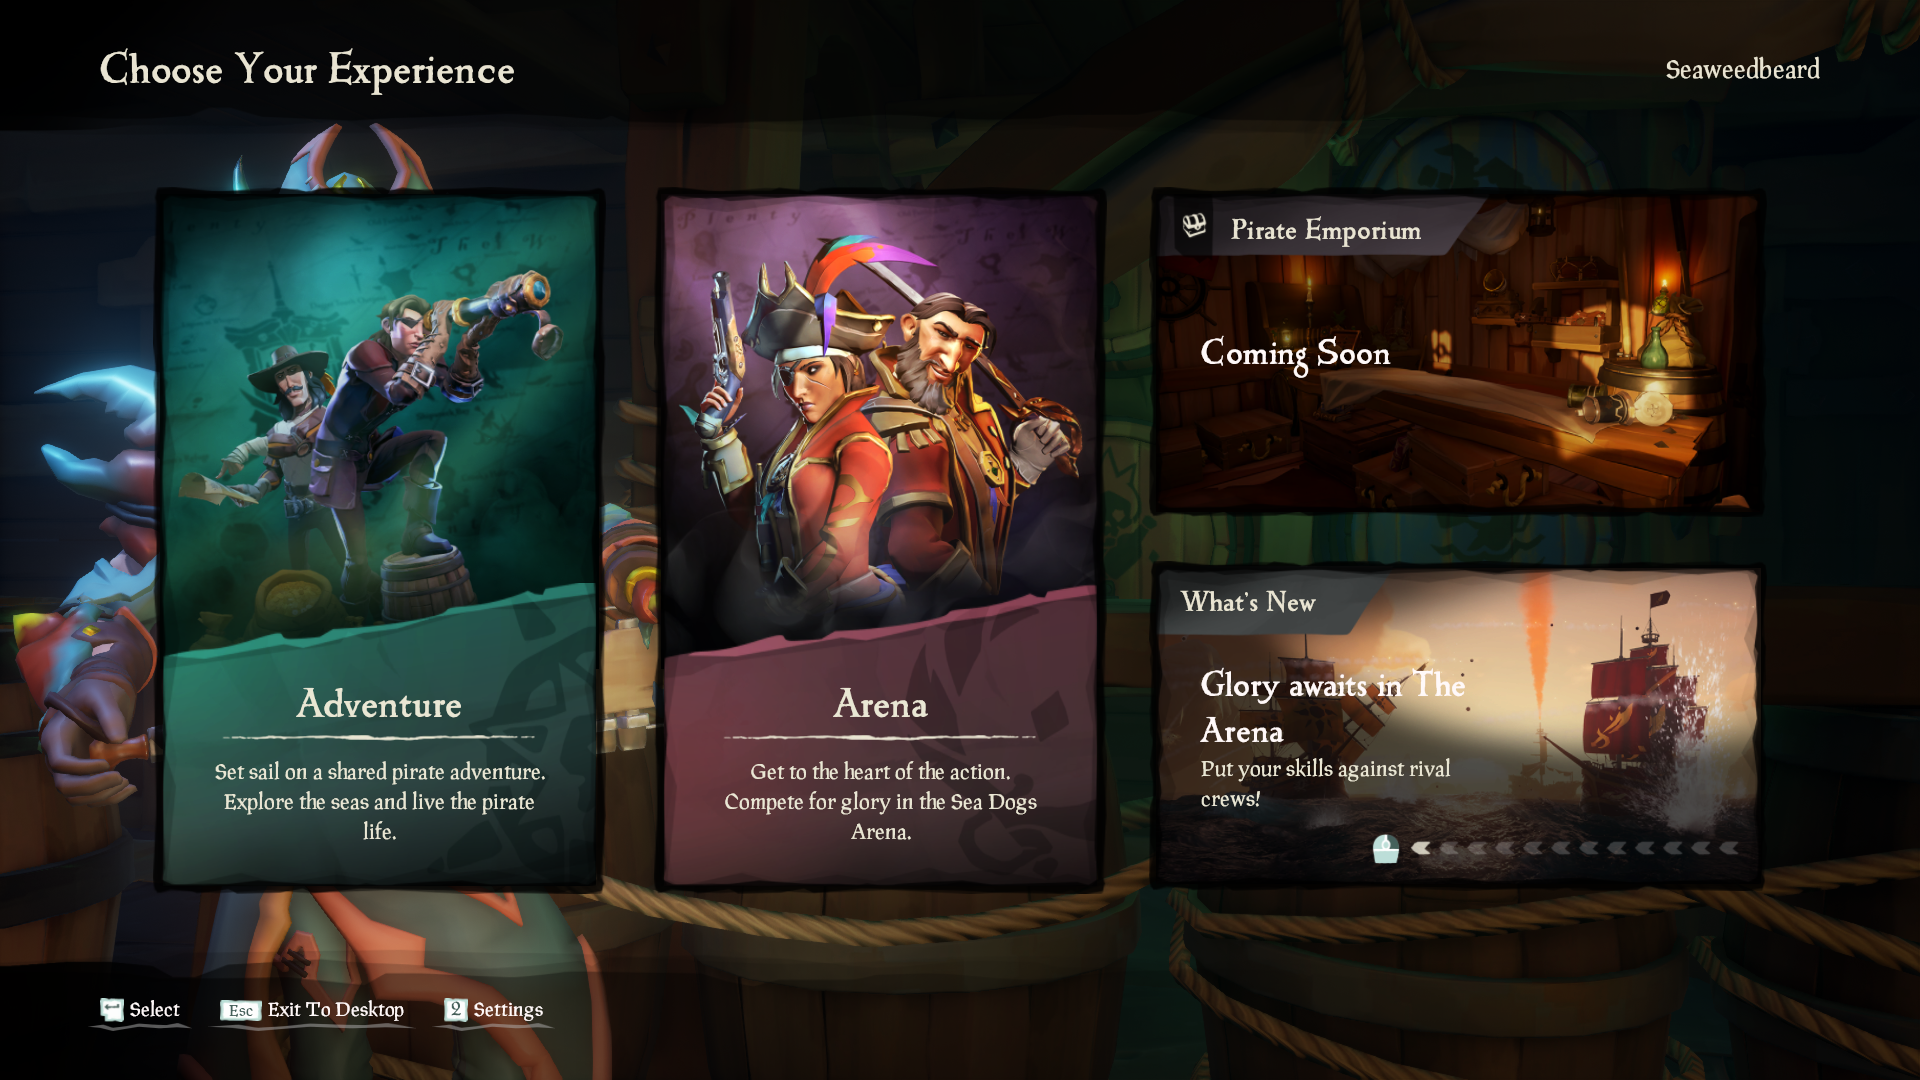
\includegraphics[scale=0.22]{img/sotmenu.png}
            \caption{Menu principal du jeu Sea of Thieves}
        \end{figure}
        \begin{figure}[hbt!]
            \centering
            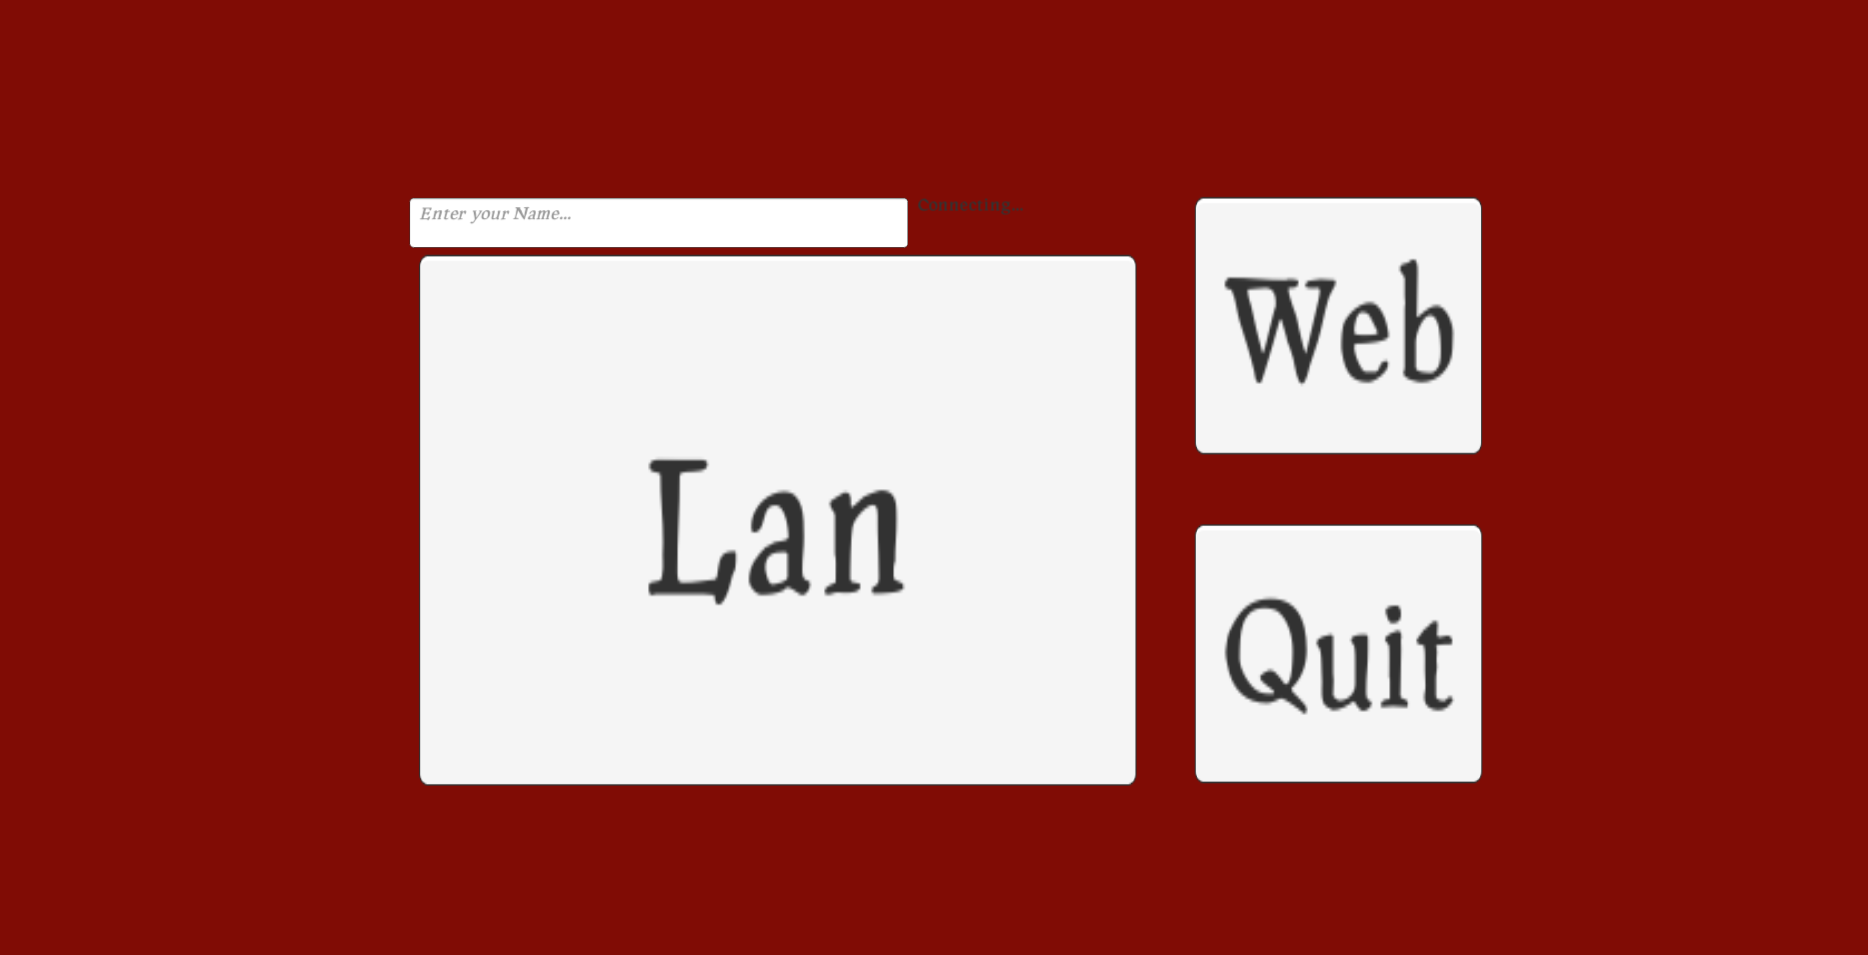
\includegraphics[scale=0.3]{img/menu.png}
            \caption{Préversion de notre menu}
        \end{figure}
        \FloatBarrier
        
        Afin de rendre le menu plus vivant, 
        nous pourrions utiliser des animations sur les boutons ainsi que sur l’arrière-plan du menu. 
        Notre menu intègrera 4 boutons et un champ. Le champ permettra au joueur d’entrer son nom dans le jeu.
        Les 4 autres boutons serviront à :
        \begin{itemize}
                \item Se connecter à une partie
                \item Quitter le jeu
                \item Régler les paramètres du jeu
                \item Personnaliser son personnage
        \end{itemize}


    \subsubsection{Première soutenance}
        
        \paragraph{Tableau des scores}

            Pendant le déroulement du jeu, le joueur a besoin de connaitre certaines informations concernant son personnage, la partie et les autres joueurs. 
            Pour fournir ces informations, nous avons opté pour un tableau des scores disponible à n’importe quel moment de la partie. Ce tableau permet également un classement simple, clair et rapide des joueurs en fonction de leurs points.
            La difficulté principale de ce tableau des scores est la synchronisation entre un script coté client qui doit actualiser à chaque pression de la touche TAB le score ainsi que la présence de chaque joueur et la récupération des données de chaque Player, mises à jour en temps réel sur le serveur.
            
            \begin{figure}[hbt!]
                    \centering
                    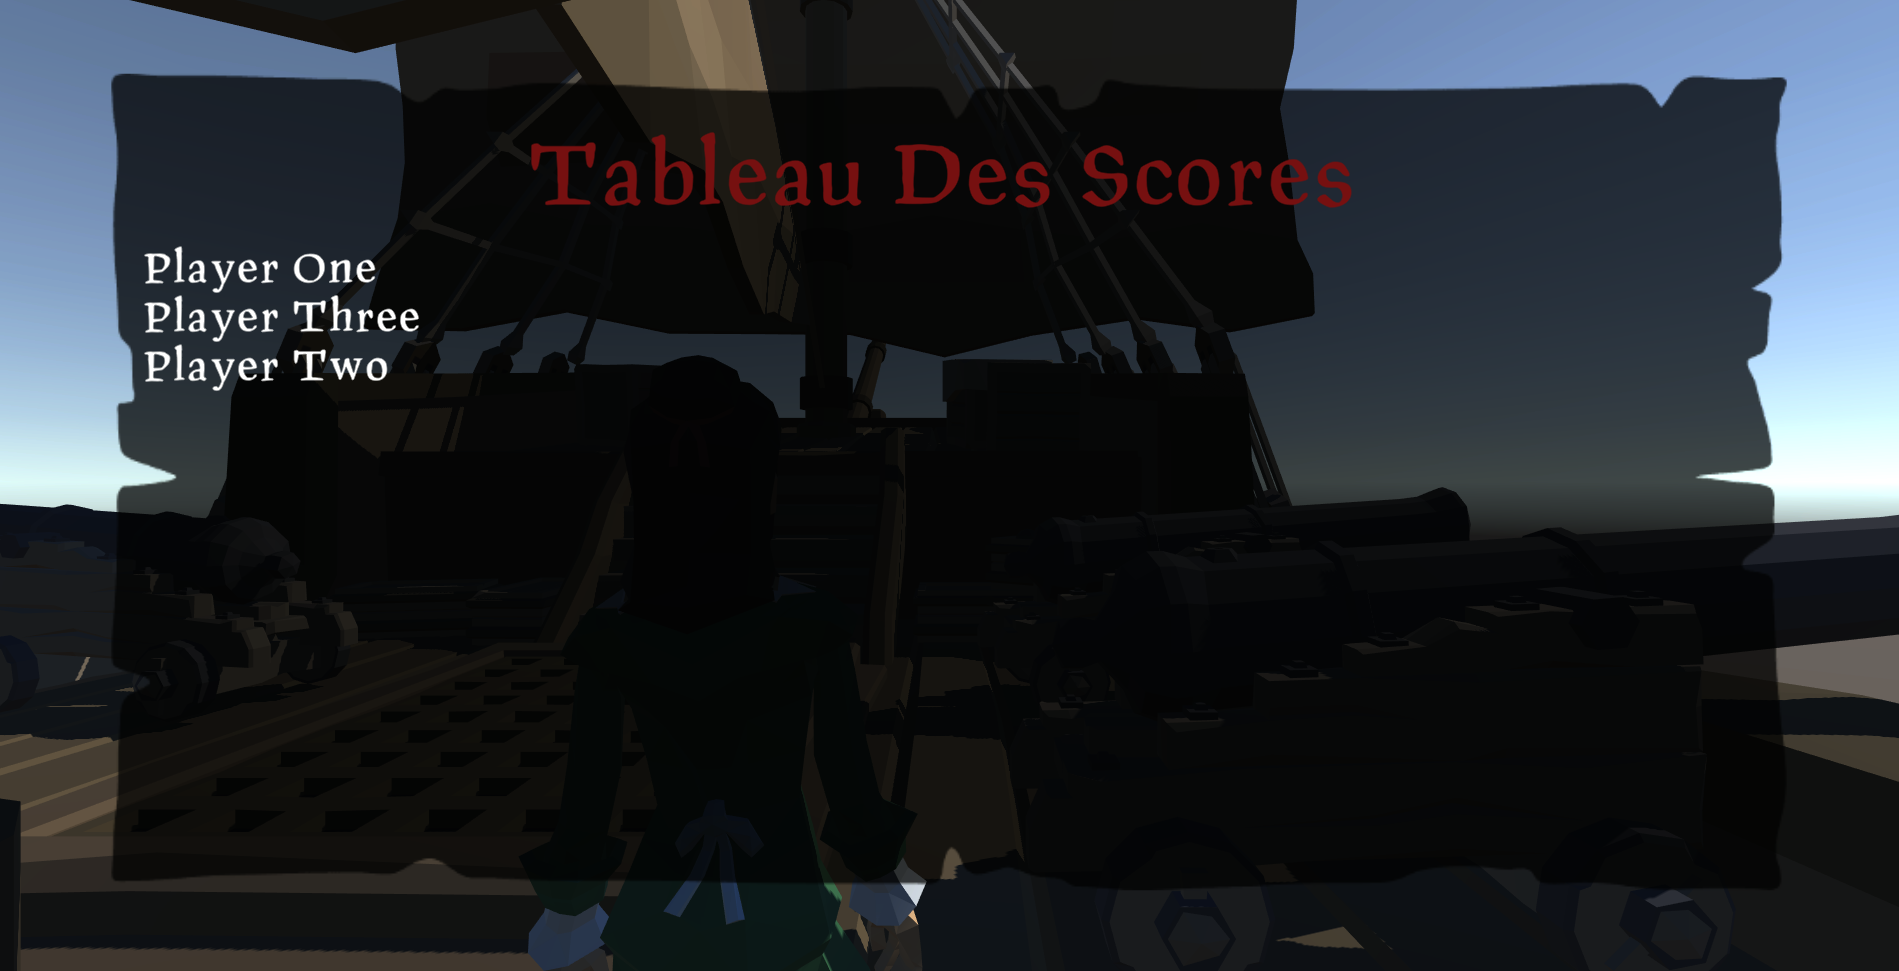
\includegraphics[scale=0.29]{img/scoreboard.PNG}
                    \caption{Première version du tableau des scores}
            \end{figure}
            \FloatBarrier


    \subsubsection{Deuxième soutenance}
    
        \paragraph{Menu principal}
        
            Le menu principal a été amélioré, afin d'y ajouter des paramètres comme la sélection du mode de fenêtre (fenêtré 
            ou plein-écran) ou le format de la fenêtre (compatible avec des formats 16:9, 4:3 et 16:10).
            Il comporte maintenant les quatre options annoncées dans le cahier des charges, à savoir jouer, modifier le personnage, 
            régler les paramètres et quitter.

            Un début de boussole a aussi implémenté, mais n'est pas accessible en jeu car encore au stade de développement. Cette dernière, 
            présente en bas à droite de l'écran, permet de localiser sa cible (avec une précision proportionnelle à la distance à la cible).

    \subsubsection{Troisième soutenance}
    
        \paragraph{Menu Principal}
        
            Le menu principal a encore été amélioré, et est maintenant très semblable à celui de Sea of Thieves, avec des boutons recouverts 
            par des images pour donner du cachet au jeu. Des danses de victoire ayant également été ajoutées au jeu, un menu de sélection est maintenant 
            disponible dans les options de configuration du joueur, au même endroit que le choix de l'apparence.
        
            \begin{figure}[hbt!]
                \centering
                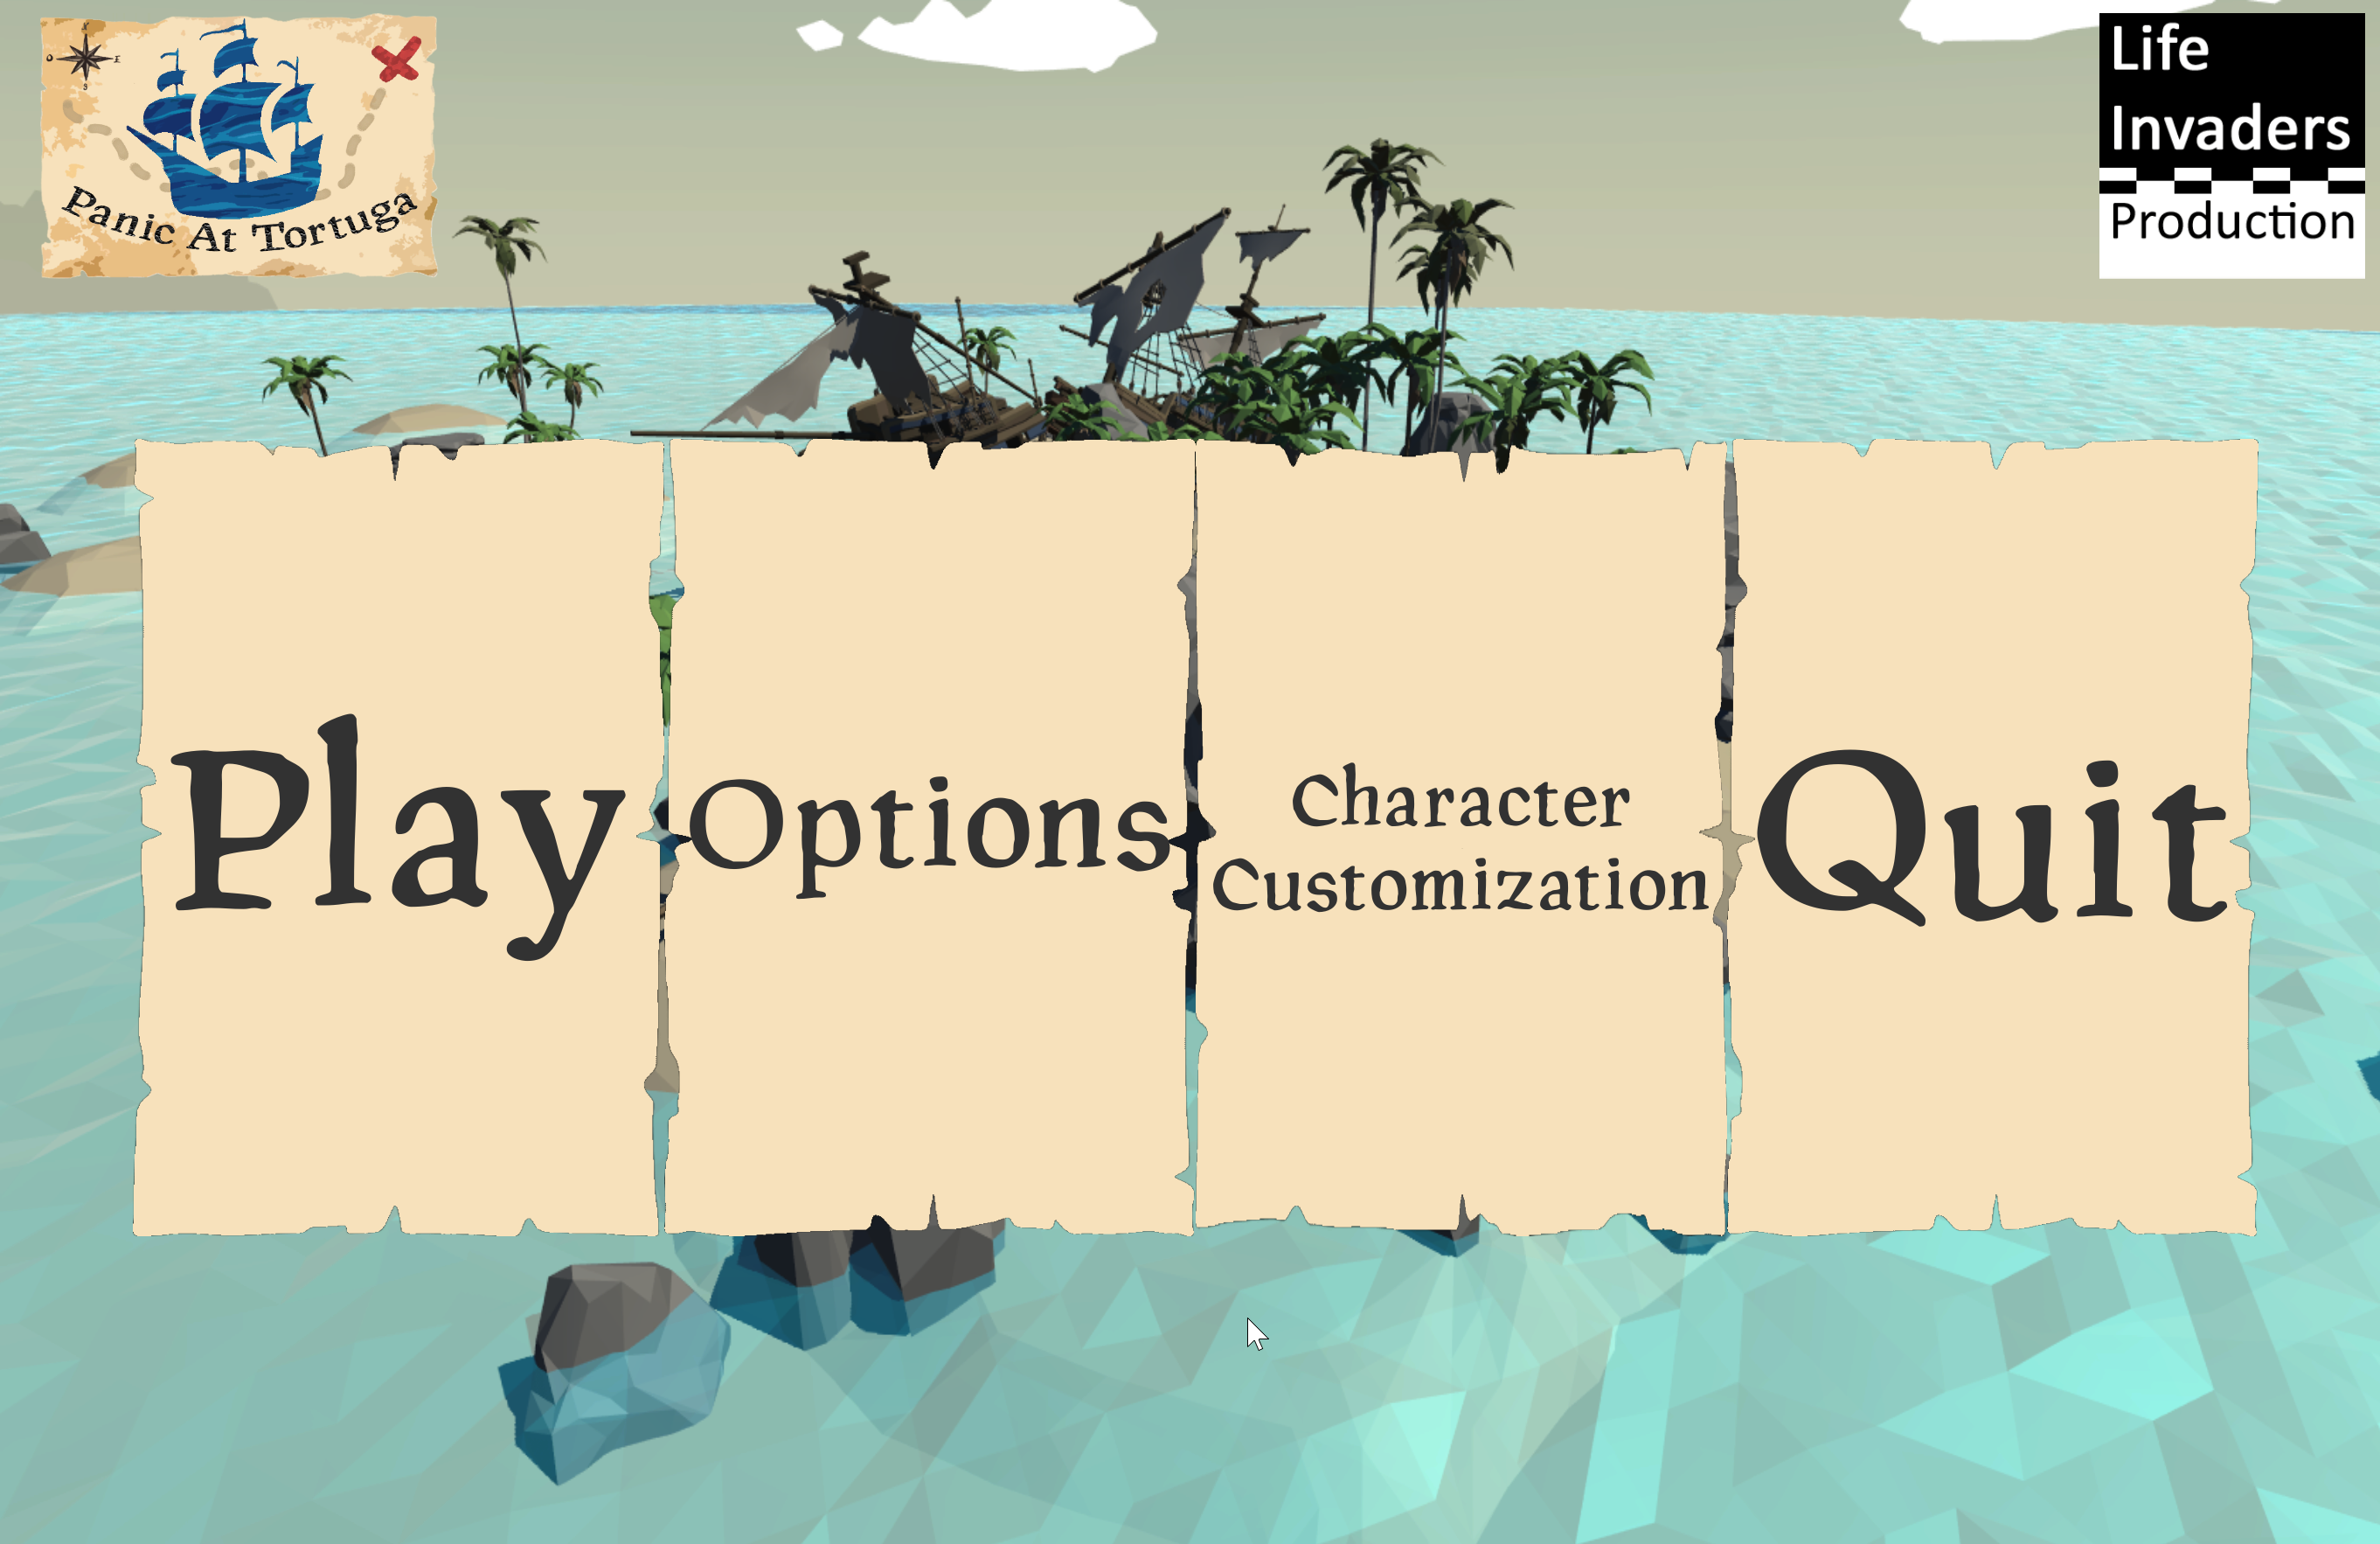
\includegraphics[scale=0.4]{img/mainmenu.png}
                \caption{Version antérieure du menu principal}
            \end{figure}

            \begin{figure}[hbt!]
                \centering
                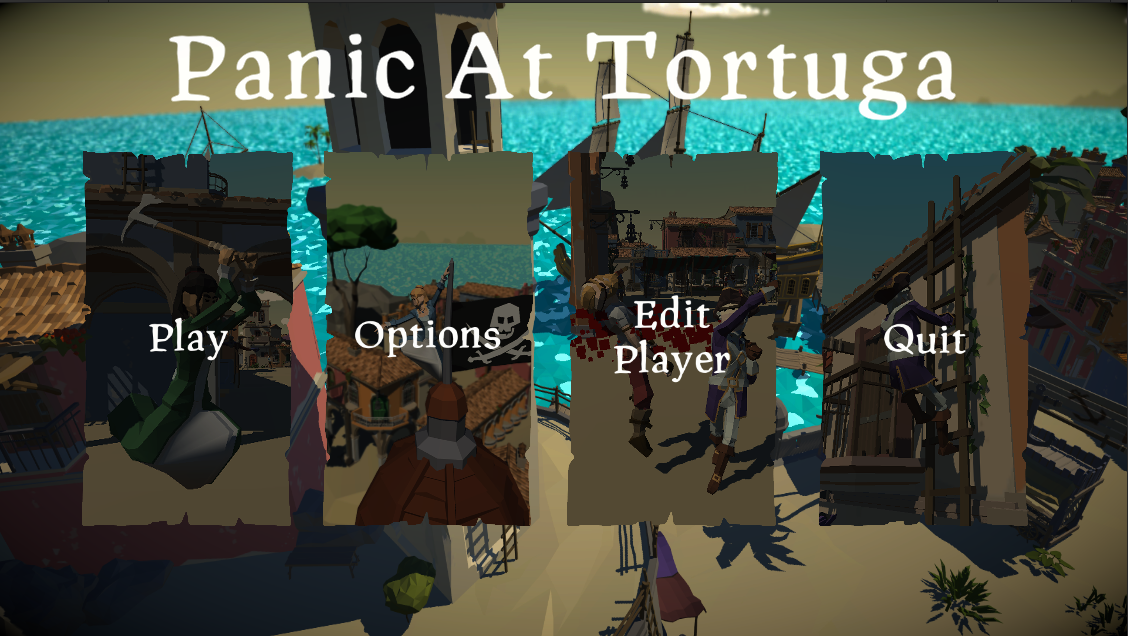
\includegraphics[scale=0.35]{img/menu_principal.png}
                \caption{Dernière version du menu}
            \end{figure}
            \FloatBarrier
        